\chapter{A Plagiarism Primer}\label{chap:plagOverview}

\section{Basic Classification of Plagiarisms}

In this part, we will try to cover common classifications of plagiarism. First, we want to figure out the purpose of 
the classification. 

There are many reasons explaining why people plagiarize. Generally those include, that they didn't have the time,
energy or the ability to do the work by themselves or that they try to steal other’s work on purpose with the hope that others
will not recognize it. This kind of plagiarism is done intentionally and named \textit{deliberate 
plagiarism}\citep{UEfAP}.

Another kind is \textit{accidental plagiarism}. This occurs when texts from some sources are copied or rephrased, but no 
reference is given. The reason is that the writer didn't know that it is a plagiarism because of \enquote{carelessness or  
lack of skill}\citep{UEfAP} while writing.

Anyway, it is important to know, that working with the source carelessly may cause plagiarism. Classification 
of plagiarism is also a good way to help distinguish typical types of plagiarism, so that people are aware and able 
to reference the sources carefully and to avoid plagiarizing.

Classification of plagiarism is also good for professors or the plagiarism detection community such as VroniPlag, because
it gives them a common terminology, which enables them to communicate faster and more efficiently. 
It also helps them to realize what category and how many percent the text is plagiarized 
if there is any suspicion, so that statistical data can be created.

% I don't understand this sentence..
So the classification is about the way to detect plagiarism while conducting a citation. But what is a citation, and 
what kinds of citation are there? Understanding of citations and the way to cite is an important thing in order to 
avoid and detect plagiarism.

\subsection{Definition of Citation}

\begin{quote}\enquote{A citation is a credit or reference to another document or source}\\ \citep{wiki:Citation}\end{quote}

According to this definition, citation is your reference to a source of information, which was generated by someone 
and should be indicated properly when this source is used in your work.

Based on \citet{Wiredprof2010}, there are 3 forms of citation:

\begin{description}
\item[Direct quotation:] \hfill \\
That is an exact word-to-word copy from one source. In this case, in order to cite you have to mark 
the text with quotation marks and indicate a  parenthetical referencing, which includes the book’s name and the page 
number where you found the source.
\item[Paraphrase:] \hfill \\
That is your own explanation of someones idea. Many people think it is not a plagiarism because the text 
is written with your own words. But it is still a plagiarism because basically that is not your idea or your opinion, 
but the author’s himself. In this case of citation, some keywords are still kept in the work. Therefore the 
parenthetical reference must be given.
\item[Summary:] \hfill \\
That is the same as paraphrase, but this kind of citation is likely a summary of the text. In this case you 
have to give the parenthetical referencing as well.
\end{description}

Now we can see that citation has a lot of forms. You are free to use the source but make sure to cite sources properly 
or you are applying a plagiarism.

After understanding what citation is and its form, now we can try to classify the plagiarism. The criteria which we 
choose for classification are based on the VroniPlag’s plagiarism categories, because this project is implemented 
based on the workflow of the VroniPlag community. 

By VroniPlag, it does not matter what citation standard system is used in the work, but it is important to know how the 
citation is documented and if the reference is given properly.

\subsubsection{VroniPlag’s classification of plagiarism}\label{sec:classification}

According to VroniPlag there are the following plagiarism categories. 
The categories are originally written in German, and the translation or the similar category in English is written 
right after the german expression.

\begin{description}
\item[Komplettplagiat/Copy \& Paste:] \hfill \\
The name of this category already indicates how the text is plagiarized. The 
plagiariser just copies from the source exactly word-by-word and does not leave any proper reference to the source 
intentionally. Some is too lazy so that they just copy existing mistakes, formats etc... without checking, which 
later can become a proof of plagiarism.

The category is differentiated by the way of conducting a citation.
Source is not cited: the original text is completely copied but the source reference is not given intentionally.
Source is cited but not completely: reference is given but not correctly.  

\item[Verschleierung/Paraphrasing:]  \hfill \\
The texts from different sources are rephrased and mixed together. The plagiariser try 
to hide his stealing by changing some word orders, replacing words with synonyms … The source is not given with the hope, 
that the text is considerably generated by the plagiariser himself and therefore the plagiarism will not be detected.

\item[Übersetzungsplagiat/translations:] \hfill \\
This kind of plagiarism occurs when the sources in foreign languages are translated. 
The plagiariser pretend that this translated text is his own work. Sources are oft not given properly. This is a 
well-liked way in researching because there are many translation tools which can be found easily in Internet such as 
Babelfish, Google Translate … and  it is not easy to detect the plagiarism with existing plagiarism detection tools.

\item[Alibi-Fußnote/The forgotten Footnote:] \hfill \\
in this category, the source is cited but the real location of the source is 
hidden.  

\item[Bauernopfer und. Verschärftes Bauernopfer:] \hfill \\
The source reference is embedded in footnote part but it redirects to 
another text part of the source which has no relation with the plagiarized text.
\end{description}

\paragraph{Other categories}


\begin{description}
\item[Halbsatzflickerei/The Labor of Laziness:] \hfill \\
The plagiariser takes sentences, or just parts of sentence from different 
sources, tries to reword them and mixes all so that they look fit together. Source reference is not or not correctly 
given.

\item[Shake \& Paste:] \hfill \\
The sentence or paragraph from one source is mixed with one from another source. This 
plagiarism can be detected by changes of writing styles. Source reference is also not given properly.
\end{description}

\section{How to detect plagiarism}
\subsection{Software systems}
\subsection{Human approach}

\section{Vroni Plag}

VroniPlag is a wiki platform which many volunteers, who are ready to give their free time, their money or 
their books/resources etc. work on. They collaborate with each other in order to detect plagiarism in dissertations or
habilitations.

VroniPlag is named after the first case which they published. The case was the one of Veronica Saß.

Because it is a wiki page, which means open to all, every one could join in. If somebody is interested in a public 
case, he can feel free to edit the page without asking for an allowance. In the chat portal of this community, one could 
ask for more help or to take a look at the list of waiting fragments.

Before starting detection, there are some information that a collaborator might know.

\subsection{Plagiarism detection steps}
A suspicious case is called \textit{candidate case}. This case is still not public for all. If a user has detected some 
suspicious part of a dissertation, he/she may first go to Chat portal to indicate his/her suspicion. He/she has 
also to give at least one original text source as proof for it. If it is well reasoned that there is an existing 
plagiarism, he/she must see if there are enough collaborators, who are ready to spend their time to work with.

The candidate case has been given an anonymous name and not public until there is proof, that there is at 
least 10\% of the pages, in which plagiarized texts are found. After that the case will be published with the 
name of the author.

During the detection process, the candidate case will be divided into smaller fragments. The fragments will be checked 
carefully if there is a plagiarism found. If there is, a report is created which shows in which fragment the 
plagiarism is found. The original source is also correspondingly given.

After checking, fragment’s state is changed to \enquote{to be proofed.} That means, this fragment must be checked again  by a 
second inspector. The result will be classified in corresponding category (see \nameref{sec:classification}).

After all fragments are checked, an overview of detected plagiarism will be generated. The overview includes the following 
parts:

\subsubsection{Part 1:} 

The whole page numbers with two different colors. The page number includes also a link redirecting to corresponding 
fragment.

\begin{itemize}
\item Grey: page in which there is no plagiarism found or not checked yet.
\item Blue: page with plagiarised texts found. The link goes to the plagiarized text in comparison with  the source as well.
\end{itemize}


\begin{figure}[!h]
  \centering
    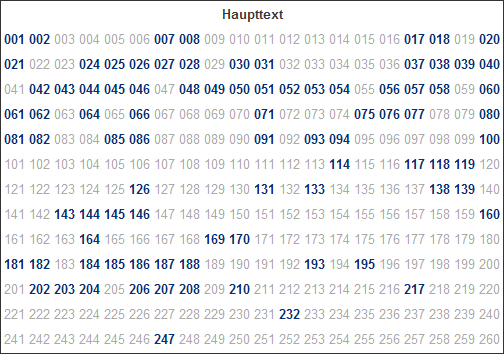
\includegraphics[width=0.95\textwidth]{images/vroni-pages.png}
  \caption{Source: \url{http://de.vroniplag.wikia.com/wiki/Lm}, 19/03/2012, 08:53}
  \label{fig:vroniPages}
\end{figure}


\subsubsection{Part 2:} 

The second part is a generated barcode label which performs the percent of plagiarism found in one page with 
different colors.

\begin{itemize}
\item Blue: pages which are not calculated in the dissertation such as Index, Appendix, literature list
\item Grey: suspiciously plagiarized
\item Black: verified that 100\% of the page is plagiarized
\item Brown: verified that more than 50\% of the page is plagiarized
\item Red: verified that more than 75\% of the page is plagiarized
\end{itemize}

\begin{figure}[!h]
  \centering
    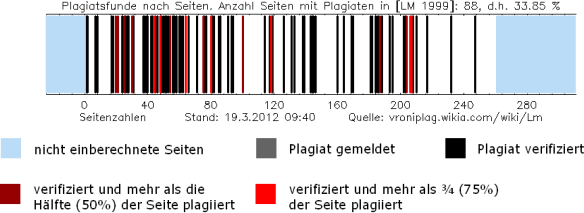
\includegraphics[width=0.95\textwidth]{images/vroni-barcode.png}
  \caption{Source: \url{http://de.vroniplag.wikia.com/wiki/Lm}, 19/03/2012, 08:54}
  \label{fig:vroniBarcode}
\end{figure}



If there is more than 10\% of the whole pages plagiarized, the case will be public on wiki. Then a report will be sent 
to the university, where the dissertation is finished.

\subsection{Technical support}

Most of the work by VroniPlag is done by hand. For example collaborators could use Google to search for sources, 
or they borrow books from the library and scan the texts. Generally there is no special software to help detect 
plagiarism, but collaborator could feel free to choose some of the existing software to help work faster.

